\section{树与二叉树}

\subsection{树的定义与基本术语}

\begin{mydef}{树}{tree}
树（Tree）是 $n\ (n\geqslant 0)$ 个结点的有限集。当 $n=0$ 时称为空树。任意一棵非空树满足：
\begin{enumerate}
    \item 有且仅有一个特定的称为\textbf{根}（Root）的结点；
    \item 当 $n>1$ 时，其余结点可分为 $m\ (m>0)$ 个互不相交的有限集 $T_1,T_2,\ldots,T_m$，其中每个集合本身又是一棵树，称为根的\textbf{子树}（Subtree）。
\end{enumerate}
树的定义是\textbf{递归}的：树由根和若干子树构成，子树本身也是树。
\end{mydef}

\begin{conclusion}{树的基本术语}{tree-terms}
\begin{itemize}
    \item \textbf{结点的度}（Degree）：结点拥有的子树个数。树的度为各结点度的最大值。
    \item \textbf{叶子结点}（Leaf）：度为 $0$ 的结点，也称终端结点。
    \item \textbf{分支结点}：度大于 $0$ 的结点，也称非终端结点。
    \item \textbf{孩子/双亲/兄弟}：结点的子树的根称为该结点的\textbf{孩子}（Child）；该结点称为孩子的\textbf{双亲}（Parent）；同一双亲的孩子互为\textbf{兄弟}（Sibling）。
    \item \textbf{路径与路径长度}：从结点 $v_0$ 到 $v_k$ 的\textbf{路径}是结点序列 $v_0,v_1,\ldots,v_k$，其中 $v_{i-1}$ 是 $v_i$ 的双亲。路径上边的数目称为\textbf{路径长度}。
    \item \textbf{深度与高度}：结点的\textbf{深度}（Depth）是从根到该结点的路径长度（根深为 $0$ 或 $1$，依约定）；树的\textbf{高度}（Height）是树中结点的最大深度。408 通常约定根深度为 $1$，高度 = 最大层数。
    \item \textbf{祖先与子孙}：从根到某结点路径上的所有结点（不含自身）为该结点的\textbf{祖先}；某结点的子树中所有结点为其\textbf{子孙}。
    \item \textbf{有序树 vs 无序树}：子树有左右次序之分则为有序树，否则为无序树。
\end{itemize}
\end{conclusion}

\begin{attention}
408 中树的\textbf{深度通常从 1 开始计数}（根的深度/层数为 1），$\text{树高} = \max\{\text{结点深度}\}$。但部分教材（如邓俊辉）从 0 开始，考试务必以题目约定为准。
\end{attention}

\begin{formula}{树的基本性质}{tree-properties}
设树 $T$ 有 $n$ 个结点，则：
\begin{enumerate}
    \item $T$ 中\textbf{边数} $= n-1$。
    \item \textbf{各结点度数之和 = 边数} $\times 2 = 2(n-1)$（无向视角），即 $\sum \deg(v) = 2(n-1)$。
    \item 从\textbf{有向}视角（父→子），$\sum \text{出度}(v) = n-1$。
    \item 设度为 $k$ 的结点有 $n_k$ 个，则 $n = \sum n_k$，且 $\sum k \cdot n_k = n-1$。
\end{enumerate}
\end{formula}

\subsection{二叉树的定义与性质}

\begin{mydef}{二叉树}{binary-tree}
二叉树（Binary Tree）是 $n\ (n\geqslant 0)$ 个结点的有限集，每个结点\textbf{至多}有两棵子树（分别称为左子树和右子树），且子树有\textbf{左右之分}，次序不能任意颠倒。
\end{mydef}

\begin{attention}
二叉树\textbf{不是}度为 2 的树——度为 2 的树要求至少有一个度为 2 的结点，而二叉树可以全部结点度为 1（如单链状）。二叉树是结点的\textbf{有限集}加上\textbf{左右子树的递归结构}，它区分左右，即使只有一棵子树也要指明是左子树还是右子树。
\end{attention}

\subsubsection{特殊二叉树}

\begin{mydef}{满二叉树}{full-binary-tree}
一棵高度为 $h$ 的二叉树，若每一层的结点数都达到最大值（第 $i$ 层有 $2^{i-1}$ 个结点，$1\leqslant i \leqslant h$），且叶子结点只出现在第 $h$ 层，则称为\textbf{满二叉树}（Full Binary Tree）。结点总数 $n = 2^h - 1$。
\end{mydef}

\begin{mydef}{完全二叉树}{complete-binary-tree}
一棵高度为 $h$、有 $n$ 个结点的二叉树，当且仅当其每个结点都与高度为 $h$ 的满二叉树中编号 $1\sim n$ 的结点\textbf{一一对应}时，称为\textbf{完全二叉树}（Complete Binary Tree）。
等价描述：除最后一层外每层都满，且最后一层的结点\textbf{从左到右}连续排列，中间不留空位。
\end{mydef}

\begin{conclusion}{完全二叉树的性质}{complete-tree-properties}
对于 $n$ 个结点的完全二叉树（层序编号 $1\sim n$）：
\begin{enumerate}
    \item 编号为 $i$ 的结点，其左孩子编号为 $2i$（若 $2i\leqslant n$，否则无左孩子）；
    \item 右孩子编号为 $2i+1$（若 $2i+1\leqslant n$，否则无右孩子）；
    \item 双亲编号为 $\lfloor i/2 \rfloor$（$i>1$）；
    \item 叶子结点只可能在最后两层出现；
    \item 若结点 $i$ 为叶子或只有左孩子，则编号 $\geqslant i$ 的结点均为叶子。
\end{enumerate}
\end{conclusion}

\subsubsection{二叉树的核心性质}

\begin{formula}{二叉树核心性质}{binary-tree-core-props}
设二叉树中度为 0、1、2 的结点数分别为 $n_0,n_1,n_2$，总结点数 $n = n_0+n_1+n_2$。
\begin{enumerate}
    \item \textbf{（408 必考）} $n_0 = n_2 + 1$。\\
    证明：由 $n = n_0+n_1+n_2$，且边数 $= n-1 = n_1 + 2n_2$（每个度为 $k$ 的结点贡献 $k$ 条边指向孩子）。联立得 $n_0 = n_2+1$。
    \item 第 $i$ 层上最多有 $2^{i-1}$ 个结点（$i\geqslant 1$）。
    \item 高度为 $h$ 的二叉树最多有 $2^h-1$ 个结点。
    \item 具有 $n$ 个结点的二叉树，高度至少为 $\lceil\log_2(n+1)\rceil$（或 $\lfloor\log_2 n\rfloor+1$）。
    \item \textbf{（408 高频）} 具有 $n$ 个结点的完全二叉树的高度为 $\lceil\log_2(n+1)\rceil$ 或 $\lfloor\log_2 n\rfloor + 1$。
\end{enumerate}
\end{formula}

\subsection{二叉树的存储结构}

\subsubsection{顺序存储结构}

\begin{formula}{二叉树的顺序存储}{seq-binary-tree}
将完全二叉树的结点按层序编号 $1\sim n$，用数组 \texttt{T[1..n]} 存储：\texttt{T[i]} 存编号为 $i$ 的结点。
\begin{lstlisting}[language=C]
#define MaxSize 100
typedef int ElemType;
typedef ElemType SqBiTree[MaxSize];  // T[0] 可闲置或存结点数
\end{lstlisting}
对于\textbf{非完全二叉树}，需要按完全二叉树的编号规则留出空位（存放特殊标记如 \texttt{0} 或 \texttt{'\#'}），会造成空间浪费。最坏情况（单链状，深度为 $k$）需要 $2^k-1$ 个存储位置，仅用 $k$ 个。
\end{formula}

\subsubsection{二叉链表存储}

\begin{formula}{二叉链表}{binary-linked-storage}
每个结点含数据域和左右指针域：
\begin{lstlisting}[language=C]
typedef struct BiTNode {
    ElemType data;
    struct BiTNode *lchild, *rchild;
} BiTNode, *BiTree;
\end{lstlisting}
$n$ 个结点的二叉链表共有 $2n$ 个指针域，其中 $n-1$ 个指向孩子（每条边对应一个指针），剩余 $n+1$ 个为空指针域。线索二叉树正是利用这些空指针域。

三叉链表：在上述结点中增加 \texttt{parent} 指针域，便于查找双亲。
\end{formula}

\begin{figure}[htbp]
\centering
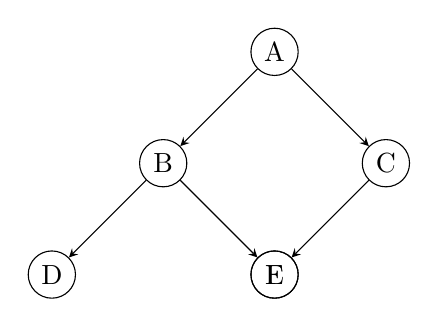
\begin{tikzpicture}[>=stealth, node distance=2.0cm, auto,
    every node/.style={draw, circle, minimum size=6mm, inner sep=1pt}]
\node (A) {A};
\node (B) [below left of=A] {B};
\node (C) [below right of=A] {C};
\node (D) [below left of=B] {D};
\node (E) [below right of=B] {E};
\node (F) [below left of=C] {F};
\draw[->] (A) -- (B);
\draw[->] (A) -- (C);
\draw[->] (B) -- (D);
\draw[->] (B) -- (E);
\draw[->] (C) -- (F);
\end{tikzpicture}
\caption{二叉树的二叉链表表示：每个结点通过 lchild/rchild 指针连接左右孩子}
\end{figure}

\subsection{二叉树的遍历}

遍历（Traversal）是按某种次序访问二叉树中的每个结点，且每个结点仅访问一次。遍历是二叉树一切操作的基础。

\subsubsection{递归遍历}

\begin{formula}{先序、中序、后序遍历的递归算法}{recursive-traversal}
三种深度优先遍历的核心区别在于\textbf{访问根结点的时机}：

\begin{lstlisting}[language=C]
// 先序遍历：根 → 左 → 右
void PreOrder(BiTree T) {
    if (T) {
        visit(T);              // ① 访问根
        PreOrder(T->lchild);   // ② 遍历左子树
        PreOrder(T->rchild);   // ③ 遍历右子树
    }
}

// 中序遍历：左 → 根 → 右
void InOrder(BiTree T) {
    if (T) {
        InOrder(T->lchild);    // ① 遍历左子树
        visit(T);              // ② 访问根
        InOrder(T->rchild);    // ③ 遍历右子树
    }
}

// 后序遍历：左 → 右 → 根
void PostOrder(BiTree T) {
    if (T) {
        PostOrder(T->lchild);  // ① 遍历左子树
        PostOrder(T->rchild);  // ② 遍历右子树
        visit(T);              // ③ 访问根
    }
}
\end{lstlisting}
\end{formula}

\begin{conclusion}{递归遍历的时间/空间复杂度}{traversal-complexity}
每个结点访问一次且仅一次：时间复杂度 $O(n)$。
递归调用栈的最大深度 = 树的高度，空间复杂度 $O(h)$，最坏情况（单链状）为 $O(n)$，平均 $O(\log n)$。
\end{conclusion}

\subsubsection{非递归遍历}

\begin{conclusion}{中序非递归遍历}{inorder-nonrecursive}
用栈模拟递归调用栈，是 408 综合应用题的高频考点：
\begin{lstlisting}[language=C]
void InOrderNR(BiTree T) {
    Stack S; InitStack(&S);
    BiTree p = T;
    while (p || !StackEmpty(S)) {
        if (p) {
            Push(&S, p);          // 沿左链走到底
            p = p->lchild;
        } else {
            Pop(&S, &p);          // 退栈，访问
            visit(p);
            p = p->rchild;        // 转向右子树
        }
    }
}
\end{lstlisting}
\textbf{核心思路：}「沿左支深入，遇空则退栈访问，再转向右子树」。这也是 408 代码题最常考察的非递归模式。
\end{conclusion}

\begin{conclusion}{先序非递归遍历}{preorder-nonrecursive}
与中序类似，但\textbf{入栈前}即访问：
\begin{lstlisting}[language=C]
void PreOrderNR(BiTree T) {
    Stack S; InitStack(&S);
    BiTree p = T;
    while (p || !StackEmpty(S)) {
        if (p) {
            visit(p);             // 先序：入栈前访问
            Push(&S, p);
            p = p->lchild;
        } else {
            Pop(&S, &p);
            p = p->rchild;
        }
    }
}
\end{lstlisting}
\end{conclusion}

\begin{conclusion}{后序非递归遍历}{postorder-nonrecursive}
后序非递归较复杂：需要区分「从左子树返回」和「从右子树返回」两种退栈情形。
\begin{lstlisting}[language=C]
void PostOrderNR(BiTree T) {
    Stack S; InitStack(&S);
    BiTree p = T, lastVisited = NULL;
    while (p || !StackEmpty(S)) {
        if (p) {
            Push(&S, p);
            p = p->lchild;           // 沿左支深入
        } else {
            GetTop(S, &p);           // 查看栈顶，不弹栈
            if (p->rchild && p->rchild != lastVisited)
                p = p->rchild;       // 右子树未访问，转向
            else {
                Pop(&S, &p);         // 左右皆访问，弹出
                visit(p);
                lastVisited = p;
                p = NULL;            // 强制下次取栈顶
            }
        }
    }
}
\end{lstlisting}
\textbf{记忆技巧：} 入栈条件同先序；退栈时必须确保右子树已访问（用 \texttt{lastVisited} 标记），否则暂不弹出。
\end{conclusion}

\subsubsection{层次遍历}

\begin{conclusion}{层次遍历}{level-order}
借助队列，逐层从左向右访问：
\begin{lstlisting}[language=C]
void LevelOrder(BiTree T) {
    Queue Q; InitQueue(&Q);
    if (T) EnQueue(&Q, T);
    while (!QueueEmpty(Q)) {
        DeQueue(&Q, &p);
        visit(p);
        if (p->lchild) EnQueue(&Q, p->lchild);
        if (p->rchild) EnQueue(&Q, p->rchild);
    }
}
\end{lstlisting}
时间复杂度 $O(n)$，空间复杂度 $O(w)$，$w$ 为树的最大宽度（最坏 $O(n)$）。
\end{conclusion}

\subsection{遍历序列构造二叉树}

\begin{conclusion}{由遍历序列构造二叉树}{construct-from-traversal}
\textbf{核心定理（408 必考）：} 已知\textbf{中序序列 + 先序序列} 或 \textbf{中序序列 + 后序序列}，可唯一确定一棵二叉树。\textbf{已知先序 + 后序无法唯一确定二叉树}（除非是完全二叉树等特殊情形）。

\textbf{构造方法}（已知先序 + 中序）：
\begin{enumerate}
    \item 先序的第一个结点为根；
    \item 在中序中找到根的位置，根左侧为左子树中序，根右侧为右子树中序；
    \item 根据左/右子树的结点数目，在先序中切分出左/右子树的先序；
    \item 对左右子树递归执行上述步骤。
\end{enumerate}

\begin{lstlisting}[language=C]
// pre[pl..pr] 为先序区间, in[il..ir] 为中序区间
BiTree Build(char pre[], char in[], int pl, int pr, int il, int ir) {
    if (pl > pr) return NULL;
    BiTree root = (BiTree)malloc(sizeof(BiTNode));
    root->data = pre[pl];                    // 根 = 先序首元
    int k;                                   // 根在中序中的位置
    for (k = il; k <= ir; k++)
        if (in[k] == pre[pl]) break;
    int leftLen = k - il;                    // 左子树结点数
    root->lchild = Build(pre, in, pl+1, pl+leftLen, il, k-1);
    root->rchild = Build(pre, in, pl+leftLen+1, pr, k+1, ir);
    return root;
}
\end{lstlisting}

后序 + 中序的构造完全对称：后序的最后结点为根，其余逻辑相同。
\end{conclusion}

\begin{attention}
408 选择题高频考察「给定两个遍历序列，判断能否唯一确定二叉树」以及「由序列还原二叉树的中间步骤」。务必掌握手动构造的流程：\textbf{找根→切分中序→切分先序/后序→递归}。
\end{attention}

\subsection{线索二叉树}

\begin{mydef}{线索二叉树}{threaded-binary-tree}
普通二叉链表中有 $n+1$ 个空指针域。线索二叉树将这些空指针域利用起来：
\begin{itemize}
    \item 若结点无左孩子，则 \texttt{lchild} 指向\textbf{前驱}（某种遍历次序下的直接前驱）；
    \item 若结点无右孩子，则 \texttt{rchild} 指向\textbf{后继}（某种遍历次序下的直接后继）。
\end{itemize}
需要两个标志位 \texttt{ltag}、\texttt{rtag} 区分指针是指向孩子（0）还是线索（1）。
\end{mydef}

\begin{formula}{线索二叉树的结点结构}{threaded-node}
\begin{lstlisting}[language=C]
typedef struct ThreadNode {
    ElemType data;
    struct ThreadNode *lchild, *rchild;
    int ltag, rtag;          // 0: 孩子指针; 1: 线索指针
} ThreadNode, *ThreadTree;
\end{lstlisting}
\end{formula}

\subsubsection{中序线索化}

\begin{conclusion}{中序线索化的算法}{inorder-threading}
在递归中序遍历的过程中，用一个\textbf{全局变量} \texttt{pre} 记录刚刚访问过的结点，以便建立线索：
\begin{lstlisting}[language=C]
ThreadNode *pre = NULL;  // 全局变量，记录前一个访问结点

void InThread(ThreadTree T) {
    if (T) {
        InThread(T->lchild);            // ① 线索化左子树
        if (!T->lchild) {               // ② 处理当前结点
            T->lchild = pre;
            T->ltag = 1;
        }
        if (pre && !pre->rchild) {      // ③ 处理前驱的右线索
            pre->rchild = T;
            pre->rtag = 1;
        }
        pre = T;                        // ④ 更新 pre
        InThread(T->rchild);            // ⑤ 线索化右子树
    }
}
\end{lstlisting}
通过增设头结点，可以将中序线索二叉树组织成循环链表以方便遍历。
\end{conclusion}

\subsubsection{线索二叉树的前驱与后继}

\begin{conclusion}{中序线索二叉树：找前驱与后继}{threaded-pred-succ}
这是 408 选择题/简答题的常考点。

\textbf{找后继 $\text{succ}(p)$：}
\begin{itemize}
    \item 若 \texttt{p->rtag == 1}，则 \texttt{p->rchild} 即为后继（线索直接给出）；
    \item 若 \texttt{p->rtag == 0}（有右孩子），后继为\textbf{右子树中第一个被访问的结点}（中序：右子树的最左下结点）。
\end{itemize}

\begin{lstlisting}[language=C]
ThreadNode *InOrderSucc(ThreadNode *p) {
    if (p->rtag == 1) return p->rchild;         // 直接由线索给出
    ThreadNode *q = p->rchild;                   // 进入右子树
    while (q->ltag == 0) q = q->lchild;          // 找到最左下结点
    return q;
}
\end{lstlisting}

\textbf{找前驱 $\text{pred}(p)$：}
\begin{itemize}
    \item 若 \texttt{p->ltag == 1}，则 \texttt{p->lchild} 即为前驱；
    \item 若 \texttt{p->ltag == 0}（有左孩子），前驱为\textbf{左子树中最后一个被访问的结点}（中序：左子树的最右下结点）。
\end{itemize}

\begin{lstlisting}[language=C]
ThreadNode *InOrderPred(ThreadNode *p) {
    if (p->ltag == 1) return p->lchild;
    ThreadNode *q = p->lchild;
    while (q->rtag == 0) q = q->rchild;
    return q;
}
\end{lstlisting}
\end{conclusion}

\begin{attention}
\textbf{408 常考陷阱：}
\begin{enumerate}
    \item 中序线索树中找前驱/后继的规律不适用于先序/后序线索树——分别有不同的查找规则。
    \item 先序线索树中找后继：有左孩子则后继为左孩子，否则为右孩子（或线索）；找前驱需要知道双亲，一般需三叉链表。
    \item 后序线索树中找前驱：有右孩子则前驱为右孩子，否则为左孩子（或线索）；找后继需要知道双亲。
\end{enumerate}
\end{attention}

\subsection{树与森林的存储与遍历}

\subsubsection{树的存储结构}

\begin{conclusion}{树的双亲表示法}{parent-representation}
用数组存储结点，每个结点附带\textbf{双亲编号}。根的双亲为 $-1$：
\begin{lstlisting}[language=C]
typedef struct {
    ElemType data;
    int parent;                // 双亲下标，-1 表示根
} PTNode;
typedef struct {
    PTNode nodes[MaxSize];
    int n;                     // 结点数
} PTree;
\end{lstlisting}
优点：求双亲 $O(1)$。缺点：求孩子需遍历整个数组 $O(n)$。
\end{conclusion}

\begin{conclusion}{孩子兄弟表示法（二叉树表示法）}{child-sibling-representation}
\textbf{408 最重要的树的存储方式：} 每个结点有两个指针：\texttt{firstchild}（指向第一个孩子）和 \texttt{nextsibling}（指向下一个兄弟）。
\begin{lstlisting}[language=C]
typedef struct CSNode {
    ElemType data;
    struct CSNode *firstchild, *nextsibling;
} CSNode, *CSTree;
\end{lstlisting}
这种表示法使得任何一棵树都可以唯一地转换为一棵二叉树——\textbf{左孩子右兄弟}。
\end{conclusion}

\subsubsection{树/森林与二叉树的转换}

\begin{conclusion}{树→二叉树的转换规则}{tree-to-binary}
给定一棵树：
\begin{enumerate}
    \item 每个结点只保留其\textbf{第一个孩子}的连线，删除与其他孩子的连线；
    \item 同一层的兄弟结点之间用新的连线连接（从左向右）；
    \item 以根为轴，将原本向下的孩子关系转为\textbf{向左下方}倾斜。
\end{enumerate}
\textbf{口诀：} 左孩子、右兄弟。转换后的二叉树右子树一定为空（因根无兄弟）。
\end{conclusion}

\begin{conclusion}{森林→二叉树的转换规则}{forest-to-binary}
\begin{enumerate}
    \item 先将森林中的每棵树各自转换为二叉树；
    \item 将第一棵树的根作为总根，后续树的根依次作为前一棵树的根的\textbf{右孩子}。
\end{enumerate}
森林转换成的二叉树，根有右子树（因为下一棵树的根成为其右孩子）。
\end{conclusion}

\subsubsection{树与森林的遍历}

\begin{conclusion}{树的遍历}{tree-traversal}
\begin{itemize}
    \item \textbf{先根遍历：} 先访问根，再依次先根遍历各子树。\textbf{结果与对应二叉树的先序遍历相同。}
    \item \textbf{后根遍历：} 先依次后根遍历各子树，再访问根。\textbf{结果与对应二叉树的中序遍历相同。}
    \item \textbf{层次遍历：} 从上到下、从左到右依次访问。
\end{itemize}
注意：树\textbf{没有中根遍历}——因为树的中序无统一定义。
\end{conclusion}

\begin{conclusion}{森林的遍历}{forest-traversal}
设森林 $F = \{T_1, T_2, \ldots, T_m\}$：
\begin{itemize}
    \item \textbf{先序遍历：} 先访问 $T_1$ 的根，再先序遍历 $T_1$ 的子树森林，最后先序遍历 $\{T_2,\ldots,T_m\}$。\textbf{结果与对应二叉树的先序遍历相同。}
    \item \textbf{中序遍历（后序遍历）：} 先中序遍历 $T_1$ 的子树森林，访问 $T_1$ 的根，再中序遍历 $\{T_2,\ldots,T_m\}$。\textbf{结果与对应二叉树的中序遍历相同。}
\end{itemize}
\textbf{结论：} 森林的先序 = 对应二叉树的先序；森林的中序 = 对应二叉树的中序。
\end{conclusion}

\subsection{Huffman 树与 Huffman 编码}

\begin{mydef}{Huffman 树}{huffman-tree}
给定 $n$ 个权值 $\{w_1,w_2,\ldots,w_n\}$ 作为 $n$ 个叶子结点的权值，构造一棵二叉树。若该树的\textbf{带权路径长度}（WPL）达到最小，则称为\textbf{最优二叉树}，即 Huffman 树。

带权路径长度定义为：
\[
\text{WPL} = \sum_{i=1}^{n} w_i \cdot l_i
\]
其中 $l_i$ 是第 $i$ 个叶子结点到根的路径长度（边的条数，或深度 $-1$）。
\end{mydef}

\begin{conclusion}{Huffman 树的构造算法}{huffman-construction}
\begin{enumerate}
    \item 将 $n$ 个权值视为 $n$ 棵仅含根结点的二叉树，构成森林 $F$；
    \item 从 $F$ 中选取\textbf{两棵根权值最小的树}作为左右子树，构造一棵新树，新树根的权值为两子树根权值之和；
    \item 将新树加入 $F$，删除原来的两棵树；
    \item 重复步骤 2—3，直到 $F$ 中只剩一棵树——即为 Huffman 树。
\end{enumerate}
可以使用\textbf{最小堆}（优先队列）高效实现：每次取出两个最小值，合并后压回。时间复杂度 $O(n\log n)$。
\end{conclusion}

\begin{formula}{Huffman 树的性质}{huffman-properties}
\begin{enumerate}
    \item Huffman 树中\textbf{没有度为 1 的结点}（$n_1=0$）。由 $n_0=n_2+1$ 得总结点数 $=2n_0-1$。
    \item 权值越大的叶子离根越近，权值越小的叶子离根越远。这是 WPL 最小化的直观体现。
    \item 给定权值集合，Huffman 树\textbf{不唯一}（左右子树可交换，等权结点次序可任意）。但 \textbf{WPL 值唯一}。
    \item Huffman 树不一定是完全二叉树。
\end{enumerate}
\end{formula}

\subsubsection{Huffman 编码}

\begin{conclusion}{Huffman 编码的构造}{huffman-encoding}
以字符出现频率为权值构造 Huffman 树，然后对每条边标记：
\begin{itemize}
    \item 从根到左孩子的边标记为 $0$；
    \item 从根到右孩子的边标记为 $1$。
\end{itemize}
从根到每个叶子结点的路径上的 $0/1$ 序列即为该字符的 Huffman 编码。

\begin{center}
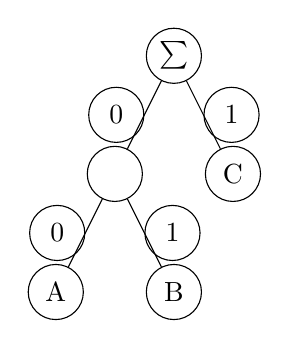
\begin{tikzpicture}[>=stealth, node distance=1.4cm and 1.8cm, auto,
    every node/.style={draw, circle, minimum size=7mm, inner sep=1pt}]
\node (R) {$\sum$}
    child { node (L) { }
        child { node (A) {A} edge from parent node[left] {0} }
        child { node (B) {B} edge from parent node[right] {1} }
        edge from parent node[left] {0}
    }
    child { node (C) {C} edge from parent node[right] {1} };
\end{tikzpicture}
\end{center}

\textbf{Huffman 编码的性质：}
\begin{enumerate}
    \item \textbf{前缀编码}（Prefix Code）：任意字符的编码都不是另一字符编码的前缀。这保证了即时解码（无需预知码长）。
    \item 由性质 1，Huffman 树中\textbf{所有字符结点都是叶子结点}，内部结点不对应任何字符。
    \item 对于同一组频率，Huffman 编码\textbf{不唯一}（由树的不唯一性导致），但总编码长度（= WPL）唯一。
\end{enumerate}
\end{conclusion}

\begin{attention}
\textbf{408 高频计算题：}
\begin{enumerate}
    \item 给定一组权值，要求\textbf{构造 Huffman 树}并画出结构图；
    \item 计算\textbf{WPL 值}（含中间步骤）；
    \item 给出 Huffman 编码方案，计算\textbf{压缩率或平均码长}；
    \item 判断某组编码是否为合法前缀编码。
\end{enumerate}
\textbf{快速计算 WPL 技巧：} 不需要等树画完再逐叶算——构造过程中\textbf{每次合并两个最小权值，将它们的和累加}，最终累加值即为 WPL。这是因为每个内部结点的权值等于其子树权值之和，所有内部结点权值之和 = WPL。
\end{attention}

\subsection{并查集}

\begin{mydef}{并查集}{union-find}
并查集（Disjoint Set / Union-Find）是一种管理\textbf{不相交集合}的数据结构，支持两种操作：
\begin{itemize}
    \item \textbf{Find(x)}：查找元素 $x$ 所属集合的代表元（根）；
    \item \textbf{Union(x, y)}：合并 $x$ 和 $y$ 所在的集合。
\end{itemize}
底层使用\textbf{树（森林）的双亲表示法}：每个集合对应一棵树，根结点为集合代表元。可用数组 \texttt{parent[i]} 存储双亲下标，根结点的 \texttt{parent} 为 $-1$。
\end{mydef}

\begin{formula}{并查集的基本实现}{union-find-impl}
\begin{lstlisting}[language=C]
#define MaxSize 100
int parent[MaxSize];

void Init(int n) {                      // 初始每个元素自成一个集合
    for (int i = 0; i < n; i++)
        parent[i] = -1;
}

int Find(int x) {                       // 查找根
    while (parent[x] >= 0)
        x = parent[x];
    return x;
}

void Union(int x, int y) {              // 合并
    int rx = Find(x), ry = Find(y);
    if (rx != ry) parent[rx] = ry;      // 将 rx 的根指向 ry
}
\end{lstlisting}
\end{formula}

\begin{conclusion}{并查集的优化}{union-find-optimizations}
朴素实现中树可能退化为链，导致 \texttt{Find} 为 $O(n)$。两种经典优化：
\begin{enumerate}
    \item \textbf{按秩合并（Union by Rank）：} 总是将高度较小的树合并到高度较大的树上，保持树高为 $O(\log n)$。可用根结点的 \texttt{parent} 值（负数）的绝对值表示秩/大小。
    \item \textbf{路径压缩（Path Compression）：} 在 \texttt{Find} 过程中，将查找路径上的所有结点直接指向根。与按秩合并结合使用时，摊还时间复杂度近乎 $O(\alpha(n))$，其中 $\alpha$ 为反 Ackermann 函数，对任何实际 $n$ 值 $\alpha(n)\leqslant 4$。
\end{enumerate}

\begin{lstlisting}[language=C]
// 路径压缩的 Find
int Find(int x) {
    if (parent[x] < 0) return x;
    return parent[x] = Find(parent[x]);   // 递归压缩
}

// 按秩合并
void Union(int x, int y) {
    int rx = Find(x), ry = Find(y);
    if (rx == ry) return;
    if (parent[rx] > parent[ry]) {         // rx 高度较小（负数绝对值较小）
        parent[ry] += parent[rx];          // 更新高度
        parent[rx] = ry;
    } else {
        parent[rx] += parent[ry];
        parent[ry] = rx;
    }
}
\end{lstlisting}
\end{conclusion}

\begin{attention}
并查集在 408 中通常以选择题（考察优化效果和时间复杂度）或简答题（结合图论中的 Kruskal 算法）出现。理解\textbf{按秩合并}和\textbf{路径压缩}的机制是重点。
\end{attention}

\subsection{408 高频考点与真题风格}

\begin{conclusion}{树与二叉树 408 选择题常考点}{tree-keypoints}
\begin{enumerate}
    \item \textbf{二叉树性质计算：} $n_0=n_2+1$ 是考察频率最高的公式，常结合 $n=n_0+n_1+n_2$ 出计算题——给定两个量求第三个。
    \item \textbf{完全二叉树的性质：} 编号规则（$2i$ 和 $2i+1$）、叶子结点个数范围、高度计算。
    \item \textbf{遍历序列分析：} 给定先序 + 中序（或后序 + 中序），还原二叉树。
    \item \textbf{线索二叉树：} 中序线索化，找前驱/后继的步骤，区分 ltag/rtag 的含义。
    \item \textbf{树/森林与二叉树的转换：} 孩子兄弟表示法，「左孩子右兄弟」规则。
    \item \textbf{Huffman 树：} WPL 计算、Huffman 树的结点数（$2n_0-1$）、给定编码判断是否为前缀码。
    \item \textbf{二叉树的遍历序列与树形对应关系：} 如前序序列与中序序列相同的树是什么形态（只有右子树的单链树）。
    \item \textbf{非递归遍历：} 中序非递归的栈变化过程，何时入栈、何时出栈。
\end{enumerate}
\end{conclusion}

\newpage
\section{习题}

\subsection{基础过关题}

\begin{enumerate}

\item \textbf{（单项选择题）} 已知一棵二叉树有 10 个度为 2 的结点，则其叶子结点个数为
\begin{center}
\begin{tabular}{ll}
(A) 9 & (B) 10 \\[6pt]
(C) 11 & (D) 无法确定
\end{tabular}
\end{center}

\item \textbf{（单项选择题）} 一棵完全二叉树共有 1001 个结点，则其叶子结点的个数为
\begin{center}
\begin{tabular}{ll}
(A) 500 & (B) 501 \\[6pt]
(C) 250 & (D) 无法确定
\end{tabular}
\end{center}

\item \textbf{（单项选择题）} 已知某二叉树的先序遍历序列为 \texttt{ABDECFG}，中序遍历序列为 \texttt{DBEAFCG}，则该二叉树的后序遍历序列为
\begin{center}
\begin{tabular}{ll}
(A) \texttt{DEBFGCA} & (B) \texttt{EDBFGCA} \\[6pt]
(C) \texttt{DEBFGAC} & (D) \texttt{DEBGFCA}
\end{tabular}
\end{center}

\item \textbf{（单项选择题）} 在具有 $n$ 个结点的二叉树中，采用二叉链表存储，空指针域的个数为
\begin{center}
\begin{tabular}{ll}
(A) $n-1$ & (B) $n$ \\[6pt]
(C) $n+1$ & (D) $2n$
\end{tabular}
\end{center}

\item \textbf{（单项选择题）} 设给定权值集合 $\{2,3,4,7,8,9\}$，构造 Huffman 树，则该树的带权路径长度 WPL 为
\begin{center}
\begin{tabular}{ll}
(A) 80 & (B) 81 \\[6pt]
(C) 82 & (D) 83
\end{tabular}
\end{center}

\item \textbf{（填空题）} 已知一棵二叉树有 $n$ 个结点，则其高度 $h$ 的取值范围是 \underline{\qquad\qquad}（设根结点的深度为 1）。

\item \textbf{（填空题）} 在中序线索二叉树中，若指针 \texttt{p} 指向某结点且 \texttt{p->rtag == 0}，则 \texttt{p} 的直接后继是 \underline{\qquad\qquad}。

\item \textbf{（简答题）} 已知一棵二叉树的先序遍历序列为 \texttt{ABDEGCF}，中序遍历序列为 \texttt{DBGEACF}。
\begin{enumerate}
    \item[(1)] 画出该二叉树的结构；
    \item[(2)] 写出其后序遍历序列；
    \item[(3)] 将该二叉树转换为对应的森林（写出转换步骤）。
\end{enumerate}

\item \textbf{（算法设计）} 设计算法求二叉树的深度（高度）。给出递归和非递归两种实现思路，并分析时间复杂度。

\item \textbf{（算法设计）} 给定一棵二叉树，设计算法判断它是否为完全二叉树。

\end{enumerate}

\subsection{真题风格与综合训练}

\begin{enumerate}[resume]

\item \textbf{（真题风格，单项选择题）} 若一棵二叉树的前序遍历序列为 \texttt{ABCDEF}，中序遍历序列为 \texttt{CBAEDF}，则后序遍历序列为
\begin{center}
\begin{tabular}{ll}
(A) \texttt{CBEFDA} & (B) \texttt{FEDCBA} \\[6pt]
(C) \texttt{CBEDFA} & (D) \texttt{不确定}
\end{tabular}
\end{center}

\item \textbf{（真题风格，单项选择题）} 设一棵 $m$ 叉树中有 $n_0$ 个度为 0 的结点，$n_1$ 个度为 1 的结点，$\ldots$，$n_m$ 个度为 $m$ 的结点，则该树中共有多少个空指针域（使用孩子链表表示，每个度为 $k$ 的结点有 $k$ 个非空指针）
\begin{center}
\begin{tabular}{ll}
(A) $n_0 + n_1 + \cdots + n_{m-1}$ & (B) $\sum_{i=1}^{m} (m-i) \cdot n_i$ \\[6pt]
(C) $\sum_{i=0}^{m-1} (m-i) \cdot n_i$ & (D) $n_1 + 2n_2 + \cdots + (m-1)n_{m-1} + 1$
\end{tabular}
\end{center}

\item \textbf{（真题风格，单项选择题）} 一组字符 $\{A,B,C,D,E\}$ 出现的频率分别为 $\{5,2,8,3,13\}$，对其进行 Huffman 编码，则字母 C 的编码可能是
\begin{center}
\begin{tabular}{ll}
(A) 00 & (B) 01 \\[6pt]
(C) 10 & (D) 11
\end{tabular}
\end{center}

\item \textbf{（真题风格，简答题）} 设中序线索二叉树的类型定义如下：
\begin{lstlisting}[language=C]
typedef struct ThreadNode {
    int data;
    struct ThreadNode *lchild, *rchild;
    int ltag, rtag;
} ThreadNode, *ThreadTree;
\end{lstlisting}
\begin{enumerate}
    \item[(1)] 编写算法，在中序线索二叉树中查找给定结点 \texttt{p} 在先序遍历下的直接后继（假设该后继存在）；
    \item[(2)] 简要说明算法的时间复杂度。
\end{enumerate}

\item \textbf{（真题风格，综合题）} 二叉树的带权路径长度（WPL）是所有叶子结点的带权路径长度之和。给定一棵二叉树，结点结构为 \texttt{[data | weight | lchild | rchild]}，其中 \texttt{weight} 为结点的权值（叶子结点有实际权值，非叶结点的 \texttt{weight} 可忽略）。
\begin{enumerate}
    \item[(1)] 编写算法计算给定二叉树的 WPL；
    \item[(2)] 分析算法的时间复杂度和空间复杂度；
    \item[(3)] 若树中只有叶子结点有权值，能否不遍历整棵树而快速得到 WPL？说明理由。
\end{enumerate}

\item \textbf{（真题风格，综合题）} 设一棵二叉树以二叉链表存储，结点结构为 \texttt{[lchild | data | rchild]}。
\begin{enumerate}
    \item[(1)] 编写非递归算法，交换二叉树中每个结点的左右子树；
    \item[(2)] 算法可否使用层次遍历实现？比较两种实现（深度优先与广度优先）在空间占用上的差异。
\end{enumerate}

\end{enumerate}

\vspace{8pt}
\noindent\textbf{拓展阅读：}
\begin{itemize}
    \item 邓俊辉《数据结构（C++语言版）》第 5 章「二叉树」——二叉树的遍历算法族（先/中/后序递归与非递归的统一框架）、Huffman 编码的贪心正确性证明。第 6 章「图」——并查集在 Kruskal 算法与图的连通性判定中的应用。
    \item Sedgewick《算法》（第 4 版）第 3.2--3.3 节「二叉查找树」与「平衡查找树」——从二叉树的遍历到 BST 上的查找与插入，为后续平衡树（AVL/红黑树）的学习建立基础。
\end{itemize}
